\documentclass[12pt]{article}
\usepackage[spanish]{babel}
\usepackage{natbib}
\usepackage{url}
\usepackage[utf8x]{inputenc}
\usepackage{amsmath}
\usepackage{float}
\usepackage{subfig}
\usepackage{graphicx}
\graphicspath{{images/}}
\usepackage{parskip}
\usepackage{fancyhdr}
\usepackage{vmargin}
\usepackage{mathtools}
\usepackage{amssymb} 



\title{Actividad \#9:Aproximación al calculo del periodo de un pendulo}							
\author{\Large Jesùs Valenzuela Nieblas\\}											
\date{\today} 

\makeatletter
\let\thetitle\@title
\let\theauthor\@author
\let\thedate\@date										
\makeatother

\pagestyle{fancy}

\lhead{\thetitle}
\cfoot{\thepage}
\rhead{}
\begin{document}

%%%%%%%%%%%%%%%%%%%%%%%%%%%%%%%%%%%%%%%%%%%%%%%%%%%%%%%%%%%%%%%%%%%%%%%%%%%%%%%%%%%%%%%%%

\begin{titlepage}
	\centering
    \vspace*{.5cm}
     
\includegraphics[scale = 0.7]{logo}\\	% University Logo
    \textsc{\Large Universidad de Sonora}\\[1.0 cm]	% University Name
	\textsc{\Large División de Ciencias Exactas y Naturales}\\[.50 cm]
  	\textsc{\Large Licenciatura en Fìsica}\\[.5 cm]
  \textsc{\large Fìsica Computacional 1}\\[1.5 cm]				% Course Name
	
	{ \huge \bfseries \thetitle}\\

    \vspace*{3 cm}
	\begin{minipage}{\textwidth}
    \centering
    \theauthor
	\end{minipage}\\[3 cm]
	
 
	\vfill
	
\end{titlepage}

%%%%%%%%%%%%%%%%%%%%%%%%%%%%%%%%%%%%%%%%%%%%%%%%%%%%%%%%%%%%%%%%%%%%%%%%%%%%%%%%%%%%%%%%%

\section{Introducciòn}
El péndulo (del lat. pendŭlus, pendiente)1 es un sistema físico que puede oscilar bajo la acción gravitatoria u otra característica física (elasticidad, por ejemplo) y que está configurado por una masa suspendida de un punto o de un eje horizontal fijos mediante un hilo, una varilla, u otro dispositivo que sirve para medir el tiempo.
El astrónomo y físico italiano Galileo Galilei observó que el periodo de oscilación es independiente de la amplitud, al menos para pequeñas oscilaciones. En cambio, aquel depende de la longitud del hilo. El período de la oscilación de un péndulo simple restringido a oscilaciones de pequeña amplitud puede aproximarse por:
\begin{equation}
T \approx 2 \pi \sqrt{\ell\over g}
\end{equation}
Para oscilaciones mayores la relación exacta para el período no es constante con la amplitud e involucra integrales elípticas de primera especie:


\begin{equation}
T = 4\sqrt{\ell\over 2g}\int^{\theta_0}_0 {1\over\sqrt{\cos\theta-\cos\theta_0}}\,d\theta
\end{equation}
Donde $\varphi_0$ es la amplitud angular máxima. La ecuación anterior puede desarrollarse en serie de Taylor obteniéndose una expresión más útil:
\begin{equation}
T = 2 \pi \sqrt{\ell\over g}
\left[1+ \left(\frac{1}{2}\right)^2\sin^2 \frac{\varphi_0}{2}+
\left(\frac{1\cdot 3}{2\cdot 4}\right)^2\sin^4 \frac{\varphi_0}{2}+
\left(\frac{1\cdot 3\cdot 5}{2\cdot 4\cdot 6}\right)^2\sin^6 \frac{\varphi_0}{2}+ \dots \right]
\end{equation}

\section{Código}

\begin{verbatim}

# coding: utf-8

# In[3]:


from scipy.integrate import quad
import numpy as np
import matplotlib.pyplot as plt


g=9.8        
l=2  


T0=2*np.pi*np.sqrt(l/g)
n=1000
e=0.0001
theta0=np.linspace(e,(np.pi)+e,n) 


#Definiendo arreglos para resultados arrojados
S=[0 for i in range(n)]
TT=[0 for i in range(n)]
R=[0 for i in range(n)]
T=[0 for i in range(n)]
real0=[0 for i in range(n)]
real2=[0 for i in range(n)]
real4=[0 for i in range(n)]
real6=[0 for i in range(n)]
real8=[0 for i in range(n)]

#------------------------------------------
#Creando doble loop para considerar los casos
#donde se agregan mas terminos de la serie de potencias


M0=0

#Comenzando un loop para poder calcular todos los resultados 
#posibles contemplando un angulo inicial variante
for i in range(M0):
    for j in range(0,n):
        F1=float(math.factorial(2*i))
        F2=float(((2**i)*(math.factorial(i)))**2)
        
        S[j]=np.sin(theta0[j]/2)**(2*i)
        TT[j]=((F1/F2)**2)*(S[j])
        R[j]=TT[j]+R[j]
        T[j]=R[j]*T0
        real0[j]=(T[j]/T0)
#------------------------------------------        
M2=2
for i in range(M2):
    for j in range(0,n):
        F1=float(math.factorial(2*i))
        F2=float(((2**i)*(math.factorial(i)))**2)
        
        S[j]=np.sin(theta0[j]/2)**(2*i)
        TT[j]=((F1/F2)**2)*(S[j])
        R[j]=TT[j]+R[j]
        T[j]=R[j]*T0
        real2[j]=(T[j]/T0)-1
#------------------------------------------        
M4=4
for i in range(M4):
    for j in range(0,n):
        F1=float(math.factorial(2*i))
        F2=float(((2**i)*(math.factorial(i)))**2)
        
        S[j]=np.sin(theta0[j]/2)**(2*i)
        TT[j]=((F1/F2)**2)*(S[j])
        R[j]=TT[j]+R[j]
        T[j]=R[j]*T0
        real4[j]=(T[j]/T0)-2
#------------------------------------------
M6=6
for i in range(M6):
    for j in range(0,n):
        F1=float(math.factorial(2*i))
        F2=float(((2**i)*(math.factorial(i)))**2)
        
        S[j]=np.sin(theta0[j]/2)**(2*i)
        TT[j]=((F1/F2)**2)*(S[j])
        R[j]=TT[j]+R[j]
        T[j]=R[j]*T0
        real6[j]=(T[j]/T0)-3
#------------------------------------------
M8=8
for i in range(M8):
    for j in range(0,n):
        F1=float(math.factorial(2*i))
        F2=float(((2**i)*(math.factorial(i)))**2)
        
        S[j]=np.sin(theta0[j]/2)**(2*i)
        TT[j]=((F1/F2)**2)*(S[j])
        R[j]=TT[j]+R[j]
        T[j]=R[j]*T0
        real8[j]=(T[j]/T0)-4

#Gráfica
plt.plot(theta0, real0, 'b',linewidth=2, label="T0")
plt.plot(theta0, real2, 'g',linewidth=2, label="T2")
plt.plot(theta0, real4, 'r',linewidth=2, label="T4")
plt.plot(theta0, real6, 'm',linewidth=2, label="T6")
plt.plot(theta0, real8, 'c',linewidth=2, label="T8")
plt.title('Error utilizando series de potencia')
plt.grid()
plt.xlabel('Angulo')
plt.xlim(0,np.pi)
plt.ylim(0,1)
plt.ylabel('Error')
plt.legend(loc='best')


fig = matplotlib.pyplot.gcf()
fig.set_size_inches(10.5,5.5)
fig.savefig('error.png',dpi=100)


\end{verbatim}
\section{Gráfica}
\begin{figure}[H]
\centering
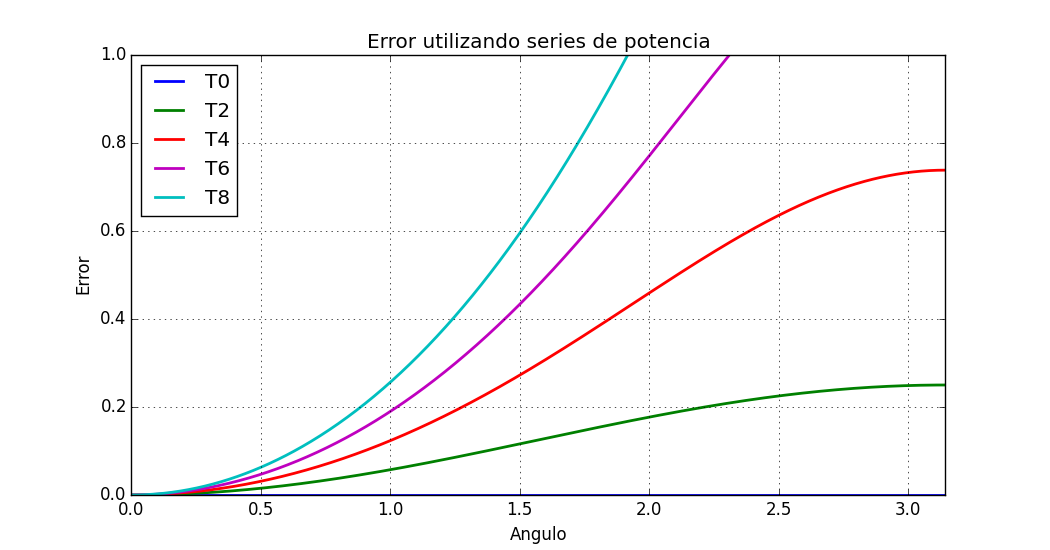
\includegraphics[scale=.7]{err}
\end{figure}

\end{document}
